\section{The True Myth}

\begin{quotex}
Art has been verified. God is the Lord, of angels, and of men---and of elves. Legend and history --- one might say, myth and historical truth --- have met and fused.
\flright{\textsc{J R R Tolkien}}

The story of Christ is simply a true myth, both factual and suggestive of meanings beyond one's grasp. \textbf{C S Lewis} redacted \end{quotex}


\paragraph{Perfect myth and perfect fact}

\begin{wrapfigure}{rt}{.3\textwidth}
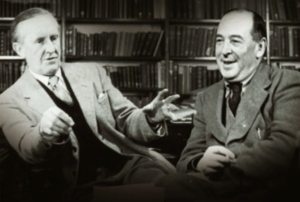
\includegraphics[width=.3\textwidth]{tolkien_and_lewis-300x202.png}
\end{wrapfigure}

Myth has come to be almost synonymous with falsehood in many minds. Rather they are stories that reveal hidden meanings. When Tolkien convinced Lewis that Christianity was a ``true myth'', the latter's life mission was changed. Since they both loved the Norse myths, the close connection between their faith and the pagan myths inspired their works. Myths are neither didactic nor allegorical, and the meaning may not be clear. Lewis wrote:

\begin{quotex}
In Pagan stories I was prepared to feel the myth as profound and suggestive of meanings beyond my grasp even tho' I could not say in cold prose ``what it meant.''
\end{quotex}

But historical facts alone provide no meaning; only very few events are worth retelling. Hence, ``sacred history'', as Rene Guenon calls it, also has meanings not always easily accessible. Lewis continued:

\begin{quotex}
The story of Christ is simply a true myth: a myth working on us in the same way as the others, but with this tremendous difference that it really happened: and one must be content to accept it in the same way, remembering that it is God's myth where the others are men's myths: i.e. the Pagan stories are God expressing Himself through the minds of poets, using such images as He found there, while Christianity is God expressing Himself through what we call ``real things'', that is, real historical events.
\end{quotex}


So, for him, pagan stories about dying and resurrecting gods reinforced his faith, the opposite effect desired by debunkers. As he put it:

\begin{quotex}
The resemblance between these myths and the Christian truth is no more accidental than the resemblance between the sun and the sun's reflection in a pond.
\flright{\textit{Reflections on the Psalms}}
\end{quotex}


Finally, he concludes:

\begin{quotex}
The heart of Christianity is a myth which is also a fact. The old myth of the Dying God, \emph{without ceasing to be myth,} comes down from the heaven of legend and imagination to the earth of history. It
\emph{happens}---at a particular date, in a particular place, followed

by definable historical consequences. We pass from a Balder or an Osiris, dying nobody knows when or where, to a historical Person crucified \emph{under Pontius Pilate}. By becoming fact it does not cease to be myth: that is the miracle. ... To be truly Christian we must both assent to the historical fact and also receive the myth with the same imaginative embrace which we accord to all myths. The one is hardly more necessary than the other.
\end{quotex}


\paragraph{Productions of the Psyche}


\begin{quotex}
Myths are first and foremost psychic phenomena that reveal the nature of the soul.
\flright{\textsc{Carl Jung}}
\end{quotex}


In opposite to the views of Lewis and Tolkien, there are the naturalizers like Joseph Campbell and Carl Jung. For them, myths are spontaneous eruptions in the collective unconscious of humankind. For proof:

\begin{quotex}
The symbols of mythology are not manufactured; they cannot be ordered, invented, or permanently suppressed. They are spontaneous productions of the psyche.
\flright{\textsc{Joseph Campbell}, \emph{The Hero with a Thousand Faces}}
\end{quotex}


Campbell doubles down on his thesis:

\begin{quotex}
These mythological symbols stem from the psyche; they speak from and to the spirit. And they are in fact the vehicles of communication between the deeper depths of our spiritual life and this relatively thin layer of consciousness by which we govern our daylight existences.
\flright{\textit{Pathways to Bliss}}
\end{quotex}


The depths of the psyche are just the subconscious, which ipso facto cannot reach the spirit. Campbell and Jung do not distinguish the subconscious from the superconscious. The subconscious tries to democratize myths, which simple observation shows to be not only false, but absurd. On the other hand, the superconscious is open to the few, i.e., the sages, prophets, seers, poets, etc., who then introduce the myths into the community. Homer and Aeneas did not repeat productions of the unconscious psyche in the manner of ethnographers organizing folklore. Rather they are visionaries who introduce the myths into the collective consciousness.

Ultimately, Campbell's position is nihilistic. The psyche is natural and hence has no access to the supernatural; to assume so is simply arbitrary. The productions of the psyche do not reveal any higher truths; at best, they make life tolerable. Campbell concedes:

\begin{quotex}
God is a metaphor for a mystery that absolutely transcends all human categories of thought, even the categories of being and non-being. Those are categories of thought. I mean it's as simple as that. So it depends on how much you want to think about it. Whether it's doing you any good. Whether it is putting you in touch with the mystery that's the ground of your own being. If it isn't, well, it's a lie. So half the people in the world are religious people who think that their metaphors are facts. Those are what we call theists. The other half are people who know that the metaphors are not facts. And so, they're lies. Those are the atheists.
\end{quotex}


\paragraph{The Law of Correspondence}


Rene Guenon agrees with Lewis and Tolkien about mythological symbols. Since they reveal higher levels of being, it is no surprise that the same symbols and myths repeat in different traditions, independent of each other. In agreement with traditional exegesis, Sacred Texts are to be interpreted on multiple levels, of which the literal or historical interpretation is just one of them. Since there are multiple levels of being, what happens on one level has a correspondence on the other levels. He explains:

\begin{quotex}
The fact is that people too often tend to think that if a symbolical meaning is admitted, the literal or historical sense must be rejected; such a view can only result from unawareness of the \textbf{Law of Correspondence} which is the very foundation of all symbolism. By virtue of this law, each thing, proceeding as it does from a metaphysical principle from which it derives all its reality, translates or expresses that principle in its own fashion and in accordance with its own order of existence, so that from one order to another all things are linked together and correspond in such a way as to contribute to the universal and total harmony, which, in the multiplicity of manifestation, can be likened to a reflection of the principia! unity itself.
\flright{\textit{Symbolism of the Cross}}
\end{quotex}


In that text, Guenon explicates the metaphysical and symbolic meaning of the Cross. Hence, we would expect that the historical life of Christ expresses such meanings. Guenon continues:

\begin{quotex}
Historical facts likewise conform to the law of correspondence, and thereby, in their own mode, translate higher realities, of which they are a human expression. We would add that from our point of view, it is this that gives to these facts the greater part of their significance. This symbolical character, while common to all historical events, is bound to be particularly clear cut in the case of events connected with what may be called ``sacred history''; thus it is recognizable in a most striking way, in all the circumstances of the life of Christ.
\end{quotex}


Finally, we see the convergence of Guenon, Lewis, and Tolkien, in Guenon's words:

\begin{quotex}
If the foregoing has been properly grasped, it will at once be apparent not only that there is no reason for denying the reality of these events and treating them as mere myths, but on the contrary that these events had to be such as they were, and could not have been otherwise; it is clearly impossible to attribute a sacred character to something devoid of all transcendent significance. In particular, if Christ died on the cross, it can be said that this was by reason of the symbolic value which the cross possesses in itself and which has always been recognized by all traditions; thus, without diminishing in any way its historical significance, the latter may be regarded as directly derived from the symbolical significance that goes with it.
\end{quotex}

For further reference, see \textit{Myth Became Fact}, by C S Lewis\footnote{\url{https://www.gornahoor.net/library/myth_became_fact.pdf}}.

\url{https://www.youtube.com/watch?v=TvnYs9FHaNk} 

\flrightit{Posted on 2022-03-27 by Cologero}

\begin{center}* * *\end{center}

\begin{footnotesize}
\begin{sffamily}
\texttt{Logres on 2022-03-29 at 16:14 said:}

This was well worth reading, extremely good. Hilariously, I came across a ``scholar's'' comments on Tolkien, fully illustrative of oblivion to what Guenon, Tolkien, Lewis, etc. would mean by ``true myth'': ``One would have thought that a scholar of Tolkien's standing could not possibly have seen the Bible and the Greek myths as instances of fairy-tales. In his epilogue to ``On Fairy-stories'', however, he actually writes, ``The Gospels contain a fairy-story, or a story of a larger kind which embraces all the essence of fairy-stories'', and he even adds that they ``contain many marvels'' (155). It will not be necessary to elaborate on the lack of sensitivity for historical contexts and genre history in this statement.'' (Dirk Vanderbeke). So, according to him, historical contexts and genre history trump any deeper inner meaning, or even (I would guess) any possibility thereof. If it's true people can't intellectualize their way to God, it's often directly because intellectualizing cuts them off from their true being in this manner, so that you can never experience something you cannot at least suspect or tentatively conceptualize, like a ``true Myth'', because you rule it out to begin with, due to bizarre concern over ``genres''.

\hfill

\texttt{yeshua21 on 2022-03-30 at 10:16 said:}

Clearly, a belief in the quasi-historical narratives can facilitate a realization of the spiritual realities to which they point and vice-versa. In by-gone days, the details of the narratives, literally construed-- garden of Eden, virgin birth, empty tomb, threats of hell, hopes of paradise --were more widely believed (and believable) and it was reasonable to demand assent. But today, I would suggest-- while such belief is still possible --it is generally counter-productive to insist on it. It is enough, it seems to me, to show respect for the tradition-- to acknowledge that it is true on the inside, where it really counts --and to continue to teach it to our children.

As I suggested awhile back, it would be nice if we could persuade those of an esoteric, gnostic bent to tolerate a more literal understanding and teaching of the tradition, while, at the same time, persuading the ``literalists'' to tolerate a more esoteric, metaphysical approach (one which acknowledges the function of mytho-poetic narratives and archetypical symbolism, regardless of their historicity). The two, together, could, as I see it, make a unified stand against ``the coarse ignorance of the masses'' and ``the moral devastation of the upper classes'' (cf. ``Regenerating Humanity'' Gornahoor).

\url{https://www.gornahoor.net/?p=13222}


Personal Testimony: ``In my mid-twenties--- immediately after my father died ---I began studying the Bible and praying with renewed intensity. But later on, I also began studying philosophy and biblical criticism and decided that I must abandon Christianity in any form since, 1) the doctrine of hell seemed inconsistent with the putative goodness and sovereignty of God; 2) the conflict between the flesh and the spirit seemed practically insurmountable; 3) historical biblical criticism seemed to undermine the veracity and authority of scripture; and 4) Nietzsche's claims--- that Christianity is false, life-denying, and morally hazardous ---seemed disturbingly plausible. But over time, I realized that I was not really at peace with that decision. As a result, when I went to graduate school, I chose a Catholic university and decided, at some point, to put my critical questions on the back burner as I resumed my pursuit of God (without insisting on knowing the end from the beginning). I concluded that whether or not the biblical narratives are really historical--- and whether or not the doctrines associated with them are entirely coherent ---they may still point (in some symbolic or mystical way) to an eternal, living reality that is both accessible and salvific, here and now.''

\url{https://jwayneferguson.wordpress.com/christian-visions/my-faith-in-christ/}


\end{sffamily}
\end{footnotesize}

